\section{Evaluation}
\label{s:eval}

\begin{table}[!ht]
 \begin{center}
 \caption{Variation in frequency and throughput with number of levels.}
\label{table1}
\begin{tabular}{ |c|c|c| }
 \hline
 Number of & Frequency ($f$) & Throughput ($\Pi$) \\
 Levels ($\beta$) & (MHz)& (GB/Sec)\\
 \hline
 \hline
 4 & 318.8 &  1.27\\
 8 & 232.8 &  1.85\\
 10 & 212 &  2.12 \\
 12 & 210 &  2.52 \\
 16 & 207.2 &  3.31\\
 20 & 173.4 &  3.46 \\
 24 & 171.6 &  4.10\\
 \hline
\end{tabular}
\end{center}
\end{table}

\begin{table}[!ht]
 \begin{center}
 \caption{Hardware cost results. LUT stands for look-up table.}
\label{table2}
\begin{tabular}{|c|c|c|c|c|}
 \hline
 Design  & Comparator  & Flip-flop & LUT &Slice \\
 \hline
 \hline
Without hole minimization & 32 & 1400 & 3165 & 4870 \\
 \hline
With hole minimization & 32 & 810 & 1970 & 2870 \\
  \hline
With hardware sharing & 16 & 750 & 1840 & 2730 \\
\hline
\end{tabular}
\end{center}
\end{table}

\begin{table}[!ht]
 \begin{center}
 \caption{Response time results.}
\label{table3}
\begin{tabular}{ |c|c|}
 \hline
 Design  &  Response Time (ms) \\
 \hline
Without hole minimization & 2010 \\
  \hline
With hole minimization & 1720 \\
  \hline
With replacement & 1337 \\
  \hline
\end{tabular}
\end{center}
\end{table}

We simulate the proposed design with ISim and implement the proposed design on the Xilinx Sparttan6 XC6SLX4 hardware platform, using 32MB on-chip memory.
We use Verilog and Python script to simulate the data path.
Through Python, we generate the test bench, which is sent to the ISim simulator.
The instruction for {\it insert/delete} is executed based on the 1-bit opcode value.
Internal logic of the FPGA determines the {\it replacement} operation based on two consecutive opcodes.
Unless otherwise stated, a random sequence of {\it insert} and {\it delete} operations is used.

\subsection{Sensitivity Analysis}
We explore how the results (frequency and throughput) change with the number of levels.
Throughput, $\Pi$, is calculated as:
\begin{eqnarray}
\Pi &=&  \frac{\omega \times  f}{\chi}
\end{eqnarray}
 where $\omega$ is the bit length, $f$ is the clock frequency, and $\chi$ is the number of clock cycles required to compute one operation.
We use the number of levels ($\beta$) and bit length ($\omega$) interchangeably.
The number of elements in the heap is $2^\omega-1 = 2^\beta -1$.

\begin{table*}
 \begin{center}
 \caption{Hardware cost and performance comparison with previous works. $n$ denotes the number of nodes.}
\label{table4}
\begin{tabular}{ |c|c|c|c|c|c|c|c|c| }
 \hline
 Design  & Comparator  & Flip-flop & SRAM & LUT &Max Frequency & Throughput ($\Pi$) & Execution & Complete \\
  & ($\kappa$)& ($F$)& ($M$) &  & ($f$) (MHz) & (GB/Sec) & Time & Tree ?\\
 \hline
 \hline
 \cite{hw8} & $2^\beta$ & $2^{\beta +1}$& 0 & 8560 & - & - & $O(1)$ & Yes\\
 \hline
 \cite{fpga2} & $2 \times \beta$ & $2^{\beta +1}$ & 0 & 1411 & - & - & $O(\log n)$ & Yes\\
 \hline
 \cite{hwsw1} & - & $2 \times \beta$ & $2 \times \beta$ & 3161 & - & - & $O(\log n)$ & No\\
 \hline
 \cite{fpga1} & $2 \times \beta$ & $2 \times \beta$ & $2 \times \beta$ & - & 180 &6.4 & $O(1)$ & No\\
 \hline
 \cite{hw2} & $2 \times \beta$ & $2 \times \beta$ & $2 \times \beta$ & - & 35.56 &10 & $O(1)$ & No\\
 \hline 
{\bf Proposed} & {\bf $\frac{\beta}{2}$} & {\bf $\beta$} & {\bf $\beta$} & {\bf 1840} & {\bf 171.6} & {\bf 4.10} & {\bf $O(1)$} & {\bf Yes}\\
 \hline
\end{tabular}
\end{center}
\end{table*}

From Table \ref{table1}, we found that the obtained clock frequency is not constant but instead inversely proportional to bit length.
We obtain a maximum frequency of 318.8 MHz from $\beta = 4$, and minimum frequency of 171.6 MHz from $\beta = 24$.
An increase in the number of levels leads to slower clock frequency but higher throughput.
As we have designed a fully pipelined architecture, the output can be obtained in each clock cycle as shown in Figure \ref{clock2}.
For the remaining experiments, we use $\beta = 24$.

\subsection{Hardware Cost and Response Time}

\begin{figure}[!ht]
  \centering
  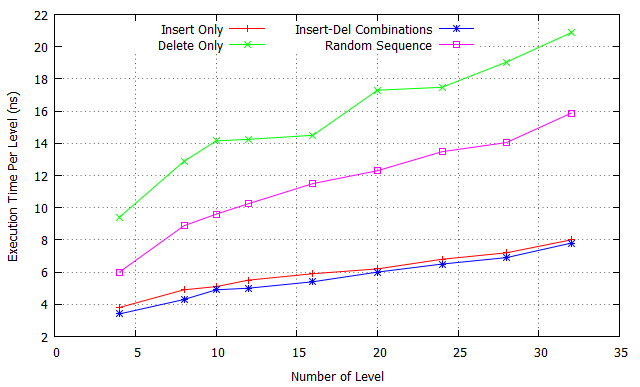
\includegraphics[width=8.8cm]{fig/random.png}
      \caption{Execution time for different sequence of operations.}
    \label{random}
\end{figure}

The hole minimization technique reduces both hardware cost and response time.
The two optimization techniques further improve them.
The hardware sharing technique contributes to the hardware cost reduction, and the {\it replacement} operation shortens the response time further.

Table~\ref{table2} shows the results of the hardware cost measurements.
Before applying the hole minimization technique, the number of comparators, flip-flops, LUTs, and slices is 32, 1400, 3165, and 4870 respectively.
Applying the technique reduces these numbers by 0.00\%, 42.14\%, 37.76\%, and 41.07\% respectively.
The hardware sharing technique reduces them even further by 50.00\%, 3.70\%, 6.60\%, and 4.88\% respectively.

The hole minimization technique also improves response time, reducing it from 2010 to 1720, which corresponds to 14.48\% reduction, as shown in Table~\ref{table3}.
Introducing the {\it replacement} operation further shortens the response time by 30.36\%.

The impact of the {\it replacement} operation depends on the sequence of operations.
Figure~\ref{random} compares the response time according to the sequence of operations.
When only insert operations come, there will be no holes created, giving us the second-best response time.
The best case is when insert-delete operations come in an alternative fashion.
In this case, the replacement operations substitute for all pairs of insert-delete operations.
The worst case is when only delete operations come right after only insert operations are processed.
In this case, none of the operations can benefit from the replacement operations.
The response time of a random sequence is between the best and worst cases.

\subsection{Comparison with Existing Techniques}

The three techniques we propose in this paper (hole minimization, hardware sharing, and replacement operation) offer a more efficient implementation of a priority queue compared to previous works.
Table~\ref{table4} compares the hardware cost and response time with existing techniques.
Since different designs address different issues and are implemented on different platforms, we make the comparison based on complexity analysis.

When compared to reference~\cite{hw8}, our design offers significantly lower overhead while achieving a similar performance level.
The number of LUTs used to implement a priority queue is reduced by 78.50\%.
The complexity of the execution time of both designs is $O(1)$.
However, while reference~\cite{hw8} requires $2^\beta$ comparators and $2^{\beta+1}$ flip-flops, our design incurs much less overhead ($\frac{\beta}{2}$ and $\beta$ respectively), offering better scalability.

Kumar {\it et. al} \cite{hwsw1} do not report neither throughput nor frequency, our design is better than their design in terms of LUT count. Moreover, it operates on $O(\log n)$ time.

Reference~\cite{fpga2} offers seemingly less overhead, but the result is, in fact, {\it underestimated}.
While reference~\cite{fpga2} is a hybrid approach combining hardware and software, the overhead in this table accounts only for hardware.
In addition, the response time of the hybrid approach is not scalable with the number of nodes.

References~\cite{fpga1,hw2} do not report the number of LUTs, but we can compare their hardware cost by complexity analysis.
They require $2 \times \beta$ comparators, flip-flops, and SRAM, whereas our design needs only $\frac{\beta}{2}$ comparators and $\beta$ flip-flops and SRAM.
The hole minimization and hardware sharing techniques have achieved aggressive optimization in hardware cost. Both the designs perform better throughput; as \cite{hw2} is implemented by using TSMC
0.35  micron CMOS standard-cell technology and \cite{fpga1} is implemented at ASIC platform.

The insert algorithm for Bhagwan and Lin's pipelined heap \cite{hw2} checks whether at least one empty node exists somewhere in the left subtree of each node the insert operation propagates through. 
If there is no empty node, the insert path moves to the right subtree. 
This means that the insert operations will always fill empty nodes starting from the left, moving down. 
Although this algorithm does guarantee that holes are {\it eventually} minimized, it does not do so in the next immediate {\it inserts}. 
It also inherently creates more holes than it minimizes and creates an imbalanced tree. 
Both of these effects waste hardware resources unless the heap is full and result in longer response time.

In comparison, insert operations in our heap always fills all nodes in each level before moving down to the next, and they fill any holes that are created immediately. Thus, our heap more efficiently uses hardware storage and has lower response time than \cite{hw2}.
